Since its commisioning in 2010, the LHC has provided experiments like CMS the opportunity to test the SM with astonishing precision. Using data collected in Runs 1 and 2, the LHC experiments have had a prolific 13 years of scientific study, boasting a combined total of roughly 3000 publications in refereed journals, with CMS contributing over 1000 physics papers to that total. Even still, theories of physics beyond the SM remain undiscovered at the LHC, with questions of Supersymmetry, Dark Matter, Grand Unification left on the table. To heighten the sensitivity of new physics searches and expand the scope of the LHC physics program, a significant upgrade to the collider is planned that will increase the integrated luminosity by a factor of ten beyond the original design. The High-Luminosity LHC (HL-LHC) is slated to begin proton-proton collisions in 2029 with the start of Run 4, kicking off Phase-2 of data-taking. Infrastructure work for the HL-LHC concluded during LS2, making way for construction of the machine in LS3 including upgrades to the quadruple magnets, cryogenics, and collimators. In addition to increased luminosity, the HL-LHC will boost the proton-proton collision energies to \SI{14}{\TeV}. 

Over the next two decades, the HL-LHC is expected to deliver an integrated luminosity of \SI{3000}{\invfb}, overshadowing the projected \SI{350}{\invfb} for Phase-1. To accumulate this much data, the collision rate inside CMS will have to be much higher than in Phase-1, which will necessarily present challenges to each subsystem. Inside CMS, the number of overlapping secondary collisions coinciding with the primary interaction, called Pile-Up (PU), averaged about 30 interactions per bunch crossing in Run 2. Specialized algorithms, such as Pile-Up Per Particle Identification (PUPPI), are used to mitigate the effects of PU. At the HL-LHC, PU within CMS may reach up to 200 interactions per bunch crossing. To reject the abundance of unwanted particles recorded in these high-PU events will require the development of more sophisticated filtering techniques and higher granularity detectors. An event display showcasing the sheer volume of particle tracks within CMS of a high-PU event can be found in Fig.~\ref{fig:highPU}. 

\begin{figure}[H]
    \centering
    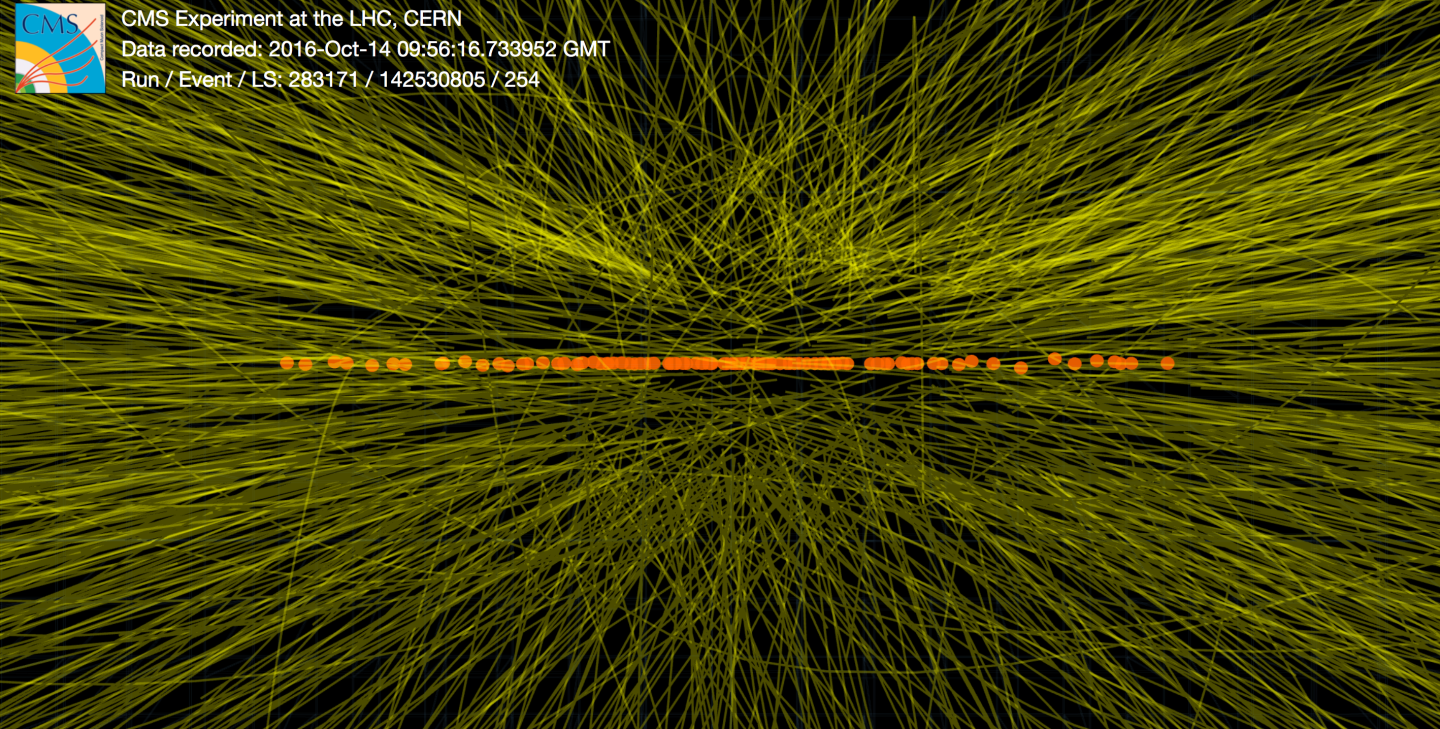
\includegraphics[width=1\textwidth]{Images/Phase2Upgrades/highpileup.png}
    \caption{An event display of a 130 PU event recorded by CMS.}
    \label{fig:highPU}
\end{figure}

The environment inside the detector throughout Phase-2 will place additional performance demands on CMS. The increase in particle flux will rapidly age current detector components, especially close to the beam pipe. Improved radiation hardness, especially of front-end detector electronics, will be required to withstand the harsh conditions. Furthermore, limited data readout bandwidth coupled with the current L1 trigger rate and latency will prove insufficient to handle the expected occupancies in Phase-2, resulting in unacceptable data loss. To cope with the challenges presented in Phase-2 of running, while profiting from the increase in luminosity, an extensive program of upgrades to the CMS subsystems was prepared and will be fully integrated prior to the first HL-LHC collisions in Run 4.
